\documentclass[varwidth=true, border=2pt]{standalone}
\usepackage{tikz}
\usetikzlibrary{shapes, calc, shapes, arrows, 3d, fadings}
\usepackage{amsmath,amssymb}

\usepackage{xcolor}
\definecolor{xvectorcolor}{HTML}{77933C}

\begin{document}
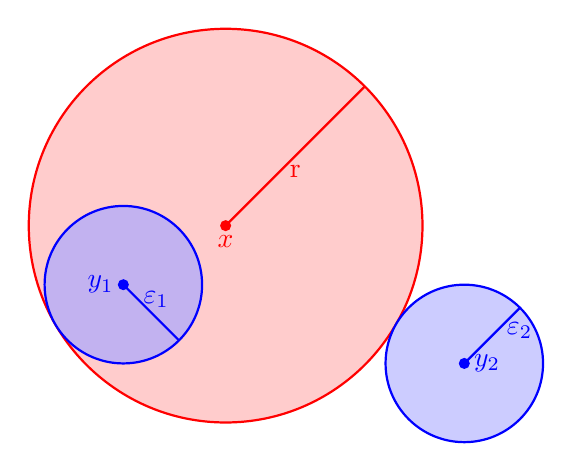
\begin{tikzpicture}
    \newcommand\radiusBig{2.5}
    \newcommand\radiusSmall{1}

    % Center for the second (outer) circle
    \path (-30:{\radiusBig+\radiusSmall}) coordinate (X);
    \path (210:{\radiusBig-\radiusSmall}) coordinate (Y);
    \path ( 0:0) coordinate (Z);

    %\fill[even odd rule,inner color=blue!70,outer color=white] (X) circle (1);
    % Lines to center
    \draw[green] (0,0) -- (X);
    \draw[green] (0,0) -- (Y);

    % The big circle
    \draw[red,thick,fill=red!20] (0,0) circle (\radiusBig); % the circle
    \draw[thick, red] (0,0) -- (45:\radiusBig);     % the radius line
    \fill[red] (Z) circle (2pt);                    % the dot
    \node (c) at ($(0,0)!0.5!(45:\radiusBig)$) [below, red] {r};
    \draw[red] (Z) node [below] {$x$};

    % The right small outer circle
    \begin{scope}[shift={(X)}]
        \node (radEnd) at (45:\radiusSmall+0.18) {};
    \end{scope}
    \draw[blue,thick,fill=blue!20] (X) circle (\radiusSmall);   % the circle
    \draw[blue,thick] (X) --  (radEnd);            % the radius line
    \fill[blue] (X) circle (2pt);                   % the dot
    \node (c) at ($(X)!0.5!(radEnd)$) [right, blue] {$\varepsilon_2$};
    \draw[blue] (X) node [right] {$y_2$};

    % The left small inner circle
    \begin{scope}[shift={(Y)}]
        \node (radEnd2) at (-45:\radiusSmall+0.18) {};
    \end{scope}
    \draw[blue,thick,fill=blue!80!red!30!white] (Y) circle (\radiusSmall);   % the circle
    \draw[blue,thick] (Y) --  (radEnd2);           % the radius line
    \fill[blue] (Y) circle (2pt);                   % the dot
    \node (c) at ($(Y)!0.5!(radEnd2)$) [above, blue] {$\varepsilon_1$};
    \draw[blue] (Y) node [left] {$y_1$};
\end{tikzpicture}
\end{document}
